\documentclass{article}
\usepackage{tikz}

\begin{document}

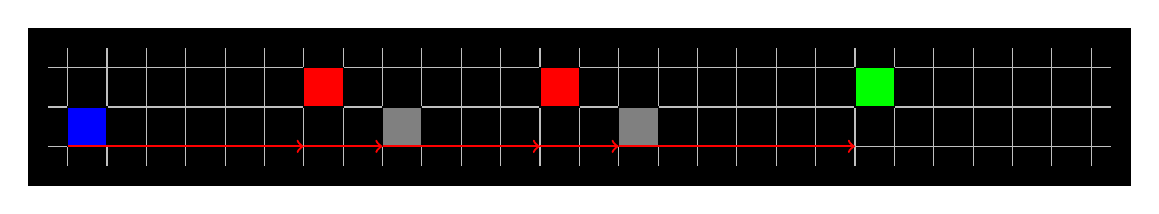
\begin{tikzpicture}[scale=0.5]
    % Draw the black walls
    \draw[fill=black] (0,0) rectangle (28,4);
    
    % Draw the grid inside the walls
    \draw[step=1, thin, gray!50] (0.5,0.5) grid (27.5,3.5);
    
    % Draw the blue start tile
    \draw[fill=blue] (1,1) rectangle ++(1,1);
    
    % Draw the red switches
    \draw[fill=red] (7,2) rectangle ++(1,1);
    \draw[fill=red] (13,2) rectangle ++(1,1);
    
    % Draw the gray doors
    \draw[fill=gray] (9,1) rectangle ++(1,1);
    \draw[fill=gray] (15,1) rectangle ++(1,1);
    
    % Draw the green final tile
    \draw[fill=green] (21,2) rectangle ++(1,1);
    
    % Draw the agent's path (assuming movement is indicated by arrows)
    \draw[->, thick, red] (1,1) -- (7,1); % Movement from blue to first red switch
    \draw[->, thick, red] (7,1) -- (9,1); % Movement through the first gray door
    \draw[->, thick, red] (9,1) -- (13,1); % Movement to the second red switch
    \draw[->, thick, red] (13,1) -- (15,1); % Movement through the second gray door
    \draw[->, thick, red] (15,1) -- (21,1); % Movement to the green end
    
\end{tikzpicture}

\end{document}